% Options for packages loaded elsewhere
\PassOptionsToPackage{unicode}{hyperref}
\PassOptionsToPackage{hyphens}{url}
%
\documentclass[
]{article}
\usepackage{amsmath,amssymb}
\usepackage{lmodern}
\usepackage{ifxetex,ifluatex}
\ifnum 0\ifxetex 1\fi\ifluatex 1\fi=0 % if pdftex
  \usepackage[T1]{fontenc}
  \usepackage[utf8]{inputenc}
  \usepackage{textcomp} % provide euro and other symbols
\else % if luatex or xetex
  \usepackage{unicode-math}
  \defaultfontfeatures{Scale=MatchLowercase}
  \defaultfontfeatures[\rmfamily]{Ligatures=TeX,Scale=1}
\fi
% Use upquote if available, for straight quotes in verbatim environments
\IfFileExists{upquote.sty}{\usepackage{upquote}}{}
\IfFileExists{microtype.sty}{% use microtype if available
  \usepackage[]{microtype}
  \UseMicrotypeSet[protrusion]{basicmath} % disable protrusion for tt fonts
}{}
\makeatletter
\@ifundefined{KOMAClassName}{% if non-KOMA class
  \IfFileExists{parskip.sty}{%
    \usepackage{parskip}
  }{% else
    \setlength{\parindent}{0pt}
    \setlength{\parskip}{6pt plus 2pt minus 1pt}}
}{% if KOMA class
  \KOMAoptions{parskip=half}}
\makeatother
\usepackage{xcolor}
\IfFileExists{xurl.sty}{\usepackage{xurl}}{} % add URL line breaks if available
\IfFileExists{bookmark.sty}{\usepackage{bookmark}}{\usepackage{hyperref}}
\hypersetup{
  pdftitle={Stat 230 HW 7},
  pdfauthor={Name:},
  hidelinks,
  pdfcreator={LaTeX via pandoc}}
\urlstyle{same} % disable monospaced font for URLs
\usepackage[margin=1in]{geometry}
\usepackage{color}
\usepackage{fancyvrb}
\newcommand{\VerbBar}{|}
\newcommand{\VERB}{\Verb[commandchars=\\\{\}]}
\DefineVerbatimEnvironment{Highlighting}{Verbatim}{commandchars=\\\{\}}
% Add ',fontsize=\small' for more characters per line
\usepackage{framed}
\definecolor{shadecolor}{RGB}{248,248,248}
\newenvironment{Shaded}{\begin{snugshade}}{\end{snugshade}}
\newcommand{\AlertTok}[1]{\textcolor[rgb]{0.94,0.16,0.16}{#1}}
\newcommand{\AnnotationTok}[1]{\textcolor[rgb]{0.56,0.35,0.01}{\textbf{\textit{#1}}}}
\newcommand{\AttributeTok}[1]{\textcolor[rgb]{0.77,0.63,0.00}{#1}}
\newcommand{\BaseNTok}[1]{\textcolor[rgb]{0.00,0.00,0.81}{#1}}
\newcommand{\BuiltInTok}[1]{#1}
\newcommand{\CharTok}[1]{\textcolor[rgb]{0.31,0.60,0.02}{#1}}
\newcommand{\CommentTok}[1]{\textcolor[rgb]{0.56,0.35,0.01}{\textit{#1}}}
\newcommand{\CommentVarTok}[1]{\textcolor[rgb]{0.56,0.35,0.01}{\textbf{\textit{#1}}}}
\newcommand{\ConstantTok}[1]{\textcolor[rgb]{0.00,0.00,0.00}{#1}}
\newcommand{\ControlFlowTok}[1]{\textcolor[rgb]{0.13,0.29,0.53}{\textbf{#1}}}
\newcommand{\DataTypeTok}[1]{\textcolor[rgb]{0.13,0.29,0.53}{#1}}
\newcommand{\DecValTok}[1]{\textcolor[rgb]{0.00,0.00,0.81}{#1}}
\newcommand{\DocumentationTok}[1]{\textcolor[rgb]{0.56,0.35,0.01}{\textbf{\textit{#1}}}}
\newcommand{\ErrorTok}[1]{\textcolor[rgb]{0.64,0.00,0.00}{\textbf{#1}}}
\newcommand{\ExtensionTok}[1]{#1}
\newcommand{\FloatTok}[1]{\textcolor[rgb]{0.00,0.00,0.81}{#1}}
\newcommand{\FunctionTok}[1]{\textcolor[rgb]{0.00,0.00,0.00}{#1}}
\newcommand{\ImportTok}[1]{#1}
\newcommand{\InformationTok}[1]{\textcolor[rgb]{0.56,0.35,0.01}{\textbf{\textit{#1}}}}
\newcommand{\KeywordTok}[1]{\textcolor[rgb]{0.13,0.29,0.53}{\textbf{#1}}}
\newcommand{\NormalTok}[1]{#1}
\newcommand{\OperatorTok}[1]{\textcolor[rgb]{0.81,0.36,0.00}{\textbf{#1}}}
\newcommand{\OtherTok}[1]{\textcolor[rgb]{0.56,0.35,0.01}{#1}}
\newcommand{\PreprocessorTok}[1]{\textcolor[rgb]{0.56,0.35,0.01}{\textit{#1}}}
\newcommand{\RegionMarkerTok}[1]{#1}
\newcommand{\SpecialCharTok}[1]{\textcolor[rgb]{0.00,0.00,0.00}{#1}}
\newcommand{\SpecialStringTok}[1]{\textcolor[rgb]{0.31,0.60,0.02}{#1}}
\newcommand{\StringTok}[1]{\textcolor[rgb]{0.31,0.60,0.02}{#1}}
\newcommand{\VariableTok}[1]{\textcolor[rgb]{0.00,0.00,0.00}{#1}}
\newcommand{\VerbatimStringTok}[1]{\textcolor[rgb]{0.31,0.60,0.02}{#1}}
\newcommand{\WarningTok}[1]{\textcolor[rgb]{0.56,0.35,0.01}{\textbf{\textit{#1}}}}
\usepackage{graphicx}
\makeatletter
\def\maxwidth{\ifdim\Gin@nat@width>\linewidth\linewidth\else\Gin@nat@width\fi}
\def\maxheight{\ifdim\Gin@nat@height>\textheight\textheight\else\Gin@nat@height\fi}
\makeatother
% Scale images if necessary, so that they will not overflow the page
% margins by default, and it is still possible to overwrite the defaults
% using explicit options in \includegraphics[width, height, ...]{}
\setkeys{Gin}{width=\maxwidth,height=\maxheight,keepaspectratio}
% Set default figure placement to htbp
\makeatletter
\def\fps@figure{htbp}
\makeatother
\setlength{\emergencystretch}{3em} % prevent overfull lines
\providecommand{\tightlist}{%
  \setlength{\itemsep}{0pt}\setlength{\parskip}{0pt}}
\setcounter{secnumdepth}{-\maxdimen} % remove section numbering
\ifluatex
  \usepackage{selnolig}  % disable illegal ligatures
\fi

\title{Stat 230 HW 7}
\author{Name:}
\date{}

\begin{document}
\maketitle

\hypertarget{worked-with}{%
\subsubsection{worked with:}\label{worked-with}}

Homework 6 is due \textbf{by 3pm Wednesday, Nov.~10}. Please complete
the assignment in this Markdown document, filling in your answers and R
code below. I didn't create answer and R chunk fields like I did with
homework 1, but please fill in your answers and R code in the same
manner as hw 1. Submit a hard copy of the \textbf{compiled pdf or word
doc} either

\begin{itemize}
\tightlist
\item
  in class
\item
  in drop-in office hours
\item
  in the paper holder outside my CMC 222 office door
\end{itemize}

Tips for using Markdown with homework sets:

\begin{itemize}
\tightlist
\item
  Work through a problem by putting your R code into R chunks in this
  .Rmd. Run the R code to make sure it works, then knit the .Rmd to
  verify they work in that environment.

  \begin{itemize}
  \tightlist
  \item
    Make sure you load your data in the .Rmd and include any needed
    \texttt{library} commands.
  \end{itemize}
\item
  Feel free to edit or delete questions, instructions, or code provided
  in this file when producing your homework solution.
\item
  For your final document, you can change the output type from
  \texttt{html\_document} to \texttt{word\_document} or
  \texttt{pdf\_document}. These two to output types are better formatted
  for printing.

  \begin{itemize}
  \tightlist
  \item
    on maize: you may need to allow for pop-ups from this site
  \end{itemize}
\item
  If you want to knit to pdf while running Rstudio from your computer
  (\emph{not} from maize), you will need a LaTeX compiler installed on
  your computer. This could be \href{https://miktex.org/}{MiKTeX},
  \href{http://www.tug.org/mactex/}{MacTeX} (mac), or TinyTex. The
  latter is installed in R: first install the R package
  \texttt{tinytex}, then run the command
  \texttt{tinytex::install\_tinytex()} to install this software.

  \begin{itemize}
  \tightlist
  \item
    If you are using maize, you don't need to install anything to knit
    to pdf!
  \end{itemize}
\end{itemize}

\begin{center}\rule{0.5\linewidth}{0.5pt}\end{center}

\hypertarget{problem-1-salk-vaccine-field-trials-of-1954}{%
\subsection{Problem 1: Salk Vaccine Field Trials of
1954}\label{problem-1-salk-vaccine-field-trials-of-1954}}

The Salk Vaccine Trial is one of the most famous, and largest, clinical
trial ever conducted. This study showed that a vaccine composed of
killed polio viruses could inoculate people against polio. Another major
outcome of this trial was to ``prove'' the benefit of
placebo-controlled, randomized experimental designs that are now the
``gold standard'' in clinical trials. In this problem you will analyze
the data from this experiment.

Experimental Design: In 11 states parents of first, second, and third
graders were asked for permission to enroll their child into the trial
(consent: 401,974 said yes and 338,778 said no). Then, of the 401,974
students who had parental consent, about half (200,745) were randomly
assigned to be injected with the vaccine while the other half (201,229)
were injected with a saline solution (vaccine: yes or no). The R
commands below give the number of polio cases (\texttt{y}) out of the
number of kids (\texttt{m}) in each combination of \texttt{consent} and
\texttt{vaccine}. Obviously, no kids were given the vaccine if they did
not have parental consent, so there are only 3 combinations of these
variables.

\begin{Shaded}
\begin{Highlighting}[]
\NormalTok{m }\OtherTok{\textless{}{-}} \FunctionTok{c}\NormalTok{(}\DecValTok{200745}\NormalTok{, }\DecValTok{201229}\NormalTok{, }\DecValTok{338778}\NormalTok{)}
\NormalTok{y }\OtherTok{\textless{}{-}} \FunctionTok{c}\NormalTok{(}\DecValTok{33}\NormalTok{,}\DecValTok{115}\NormalTok{,}\DecValTok{121}\NormalTok{)}
\NormalTok{consent}\OtherTok{\textless{}{-}} \FunctionTok{c}\NormalTok{(}\StringTok{"yes"}\NormalTok{,}\StringTok{"yes"}\NormalTok{,}\StringTok{"no"}\NormalTok{)}
\NormalTok{vaccine }\OtherTok{\textless{}{-}} \FunctionTok{c}\NormalTok{(}\StringTok{"yes"}\NormalTok{,}\StringTok{"no"}\NormalTok{,}\StringTok{"no"}\NormalTok{)}
\NormalTok{salk}\OtherTok{\textless{}{-}} \FunctionTok{data.frame}\NormalTok{(m,y,consent,vaccine)}
\NormalTok{salk}
\NormalTok{       m   y consent vaccine}
\DecValTok{1} \DecValTok{200745}  \DecValTok{33}\NormalTok{     yes     yes}
\DecValTok{2} \DecValTok{201229} \DecValTok{115}\NormalTok{     yes      no}
\DecValTok{3} \DecValTok{338778} \DecValTok{121}\NormalTok{      no      no}
\end{Highlighting}
\end{Shaded}

\hypertarget{a-fit-the-binomial-logistic-regression-of-y-on-consent-and-vaccine.-after-accounting-for-parental-consent-what-effect-does-the-vaccine-have-on-the-odds-of-getting-polio-compute-and-interpret-a-95-confidence-interval-for-this-effect.-note-that-this-is-a-causal-effect-since-the-vaccine-was-randomly-assigned-to-consenting-kids.}{%
\subsubsection{\texorpdfstring{(1a) Fit the binomial logistic regression
of \texttt{y} on \texttt{consent} and \texttt{vaccine}. After accounting
for parental consent, what effect does the vaccine have on the odds of
getting polio? Compute and interpret a 95\% confidence interval for this
effect. (Note that this is a causal effect since the vaccine was
randomly assigned to consenting
kids.)}{(1a) Fit the binomial logistic regression of y on consent and vaccine. After accounting for parental consent, what effect does the vaccine have on the odds of getting polio? Compute and interpret a 95\% confidence interval for this effect. (Note that this is a causal effect since the vaccine was randomly assigned to consenting kids.)}}\label{a-fit-the-binomial-logistic-regression-of-y-on-consent-and-vaccine.-after-accounting-for-parental-consent-what-effect-does-the-vaccine-have-on-the-odds-of-getting-polio-compute-and-interpret-a-95-confidence-interval-for-this-effect.-note-that-this-is-a-causal-effect-since-the-vaccine-was-randomly-assigned-to-consenting-kids.}}

\begin{Shaded}
\begin{Highlighting}[]
\NormalTok{salk\_glm }\OtherTok{\textless{}{-}} \FunctionTok{glm}\NormalTok{(y}\SpecialCharTok{/}\NormalTok{m }\SpecialCharTok{\textasciitilde{}}\NormalTok{ consent }\SpecialCharTok{+}\NormalTok{ vaccine, }\AttributeTok{family =} \StringTok{"binomial"}\NormalTok{, }\AttributeTok{weights =}\NormalTok{ m , }\AttributeTok{data=}\NormalTok{ salk)}
\FunctionTok{tidy}\NormalTok{(salk\_glm, }\AttributeTok{conf.int=}\ConstantTok{TRUE}\NormalTok{)}
\CommentTok{\# A tibble: 3 x 7}
\NormalTok{  term        estimate std.error statistic  p.value conf.low conf.high}
  \SpecialCharTok{\textless{}}\NormalTok{chr}\SpecialCharTok{\textgreater{}}          \ErrorTok{\textless{}}\NormalTok{dbl}\SpecialCharTok{\textgreater{}}     \ErrorTok{\textless{}}\NormalTok{dbl}\SpecialCharTok{\textgreater{}}     \ErrorTok{\textless{}}\NormalTok{dbl}\SpecialCharTok{\textgreater{}}    \ErrorTok{\textless{}}\NormalTok{dbl}\SpecialCharTok{\textgreater{}}    \ErrorTok{\textless{}}\NormalTok{dbl}\SpecialCharTok{\textgreater{}}     \ErrorTok{\textless{}}\NormalTok{dbl}\SpecialCharTok{\textgreater{}}
\DecValTok{1}\NormalTok{ (Intercept)   }\SpecialCharTok{{-}}\FloatTok{7.94}     \FloatTok{0.0909}    \SpecialCharTok{{-}}\FloatTok{87.3}  \DecValTok{0}          \SpecialCharTok{{-}}\FloatTok{8.12}     \SpecialCharTok{{-}}\FloatTok{7.76} 
\DecValTok{2}\NormalTok{ consentyes     }\FloatTok{0.470}    \FloatTok{0.130}       \FloatTok{3.61} \FloatTok{3.06}\NormalTok{e}\SpecialCharTok{{-}} \DecValTok{4}    \FloatTok{0.214}     \FloatTok{0.726}
\DecValTok{3}\NormalTok{ vaccineyes    }\SpecialCharTok{{-}}\FloatTok{1.25}     \FloatTok{0.198}      \SpecialCharTok{{-}}\FloatTok{6.31} \FloatTok{2.78e{-}10}   \SpecialCharTok{{-}}\FloatTok{1.65}     \SpecialCharTok{{-}}\FloatTok{0.872}
\end{Highlighting}
\end{Shaded}

\[odds(consent,vaccine) = e^{-7.9369525 + 0.4702575(consentyes) - 1.2464237(vaccineyes)} = e^{-7.9369525}e^{0.4702575(consentyes)}e^{-1.2464237(vaccineyes)}\]
\[odds(vaccineyes = 1) = e^{-1.2464237(1)} = 0.2875313\]

With parental consent, the vaccine results in a multiplicative change of
0.2875313 (meaning that the vaccine decreases the odss of getting polio
by 71.24687\%) (95\% CI from 58.2\$ to 80.8\%)

\hypertarget{b-after-accounting-for-vaccine-treatment-what-effect-does-parental-consent-have-on-the-odds-of-getting-polio-compute-and-interpret-a-95-confidence-interval-for-this-effect.-note-that-this-is-not-a-causal-effect-since-parental-consent-was-not-randomly-assigned-to-kids.}{%
\subsubsection{(1b) After accounting for vaccine treatment, what effect
does parental consent have on the odds of getting polio? Compute and
interpret a 95\% confidence interval for this effect. (Note that this is
not a causal effect since parental consent was not randomly assigned to
kids.)}\label{b-after-accounting-for-vaccine-treatment-what-effect-does-parental-consent-have-on-the-odds-of-getting-polio-compute-and-interpret-a-95-confidence-interval-for-this-effect.-note-that-this-is-not-a-causal-effect-since-parental-consent-was-not-randomly-assigned-to-kids.}}

\[odds(consentyes = 1) = e^{0.4702575(1)} = 1.600406\]

After vaccine treatment, parental consent has a 1.600406 multiplicative
factor on the odds of the child getting polio. Meaning that parental
consent leads to a 60\% increase of the chance for their child to get
polio. (95\% CI from 23.9\% to 106.6\%)

\hypertarget{c-some-details-about-polio-researchers-knew-that-when-raised-in-unsanitary-conditions-babies-could-actually-build-a-natural-immunity-to-polio-when-mildly-exposed-to-it.-this-immunity-made-them-less-susceptible-to-the-severe-strain-of-the-disease-as-they-grow.-children-who-were-protected-from-this-exposure-by-clean-surroundings-did-not-usually-build-this-immunity-and-were-more-likely-to-get-the-disease.-demographic-data-collected-during-the-experiment-showed-that-kids-with-no-parental-consent-had-similar-family-backgrounds.-records-showed-that-these-kids-tended-to-come-from-lower-income-households-compared-to-kids-whose-parents-did-consent.-use-this-information-to-try-to-explain-the-parental-consent-effect-you-quantified-in-part-b.}{%
\subsubsection{(1c) Some details about polio: Researchers knew that when
raised in unsanitary conditions, babies could actually build a natural
immunity to polio when mildly exposed to it. This immunity made them
less susceptible to the severe strain of the disease as they grow.
Children who were protected from this exposure by clean surroundings did
not usually build this immunity and were more likely to get the disease.
Demographic data collected during the experiment showed that kids with
no parental consent had similar family backgrounds. Records showed that
these kids tended to come from lower income households compared to kids
whose parents did consent. Use this information to try to explain the
parental consent effect you quantified in part
(b).}\label{c-some-details-about-polio-researchers-knew-that-when-raised-in-unsanitary-conditions-babies-could-actually-build-a-natural-immunity-to-polio-when-mildly-exposed-to-it.-this-immunity-made-them-less-susceptible-to-the-severe-strain-of-the-disease-as-they-grow.-children-who-were-protected-from-this-exposure-by-clean-surroundings-did-not-usually-build-this-immunity-and-were-more-likely-to-get-the-disease.-demographic-data-collected-during-the-experiment-showed-that-kids-with-no-parental-consent-had-similar-family-backgrounds.-records-showed-that-these-kids-tended-to-come-from-lower-income-households-compared-to-kids-whose-parents-did-consent.-use-this-information-to-try-to-explain-the-parental-consent-effect-you-quantified-in-part-b.}}

Since the kids who's parents who did not give consent to the vaccine
have tended to live in lower income households, they were more likely to
have built a natural immunity against polio when mildly exposed. As
such, even without parental consent some of the kids can still be
considered to have a ``pseudo vaccine'' through this exposure. As such,
the parental consent effect in part (b) is somewhat mitigated by the
fact that their kids have most likely built up a resistance to polio
from living in a low-income background. Also, the parents who did
consent to the vaccine, half of them got a placebo (saline solution)
instead of the actual vaccine, which also accounts for why those who
consented and did not get the vaccine to have a higher chance of getting
polio.

\begin{center}\rule{0.5\linewidth}{0.5pt}\end{center}

\hypertarget{problem-2-vitamin-c-chapter-21-exercise-12-a-c}{%
\subsection{Problem 2: Vitamin C Chapter 21 exercise 12
(a-c)}\label{problem-2-vitamin-c-chapter-21-exercise-12-a-c}}

You'll need to enter the data for this example by hand. You can use code
similar to that used in Problem 2 above to do so.

\begin{enumerate}
\def\labelenumi{\alph{enumi}.}
\item
  \newline
\end{enumerate}

\begin{Shaded}
\begin{Highlighting}[]
\NormalTok{m }\OtherTok{\textless{}{-}} \FunctionTok{c}\NormalTok{(}\DecValTok{411}\NormalTok{, }\DecValTok{407}\NormalTok{)}
\NormalTok{y }\OtherTok{\textless{}{-}} \FunctionTok{c}\NormalTok{(}\DecValTok{335}\NormalTok{,}\DecValTok{302}\NormalTok{)}
\NormalTok{placebo }\OtherTok{\textless{}{-}} \FunctionTok{c}\NormalTok{(}\StringTok{"yes"}\NormalTok{,}\StringTok{"no"}\NormalTok{)}
\NormalTok{ex2112 }\OtherTok{\textless{}{-}} \FunctionTok{data.frame}\NormalTok{(m,y,placebo)}
\NormalTok{ex2112}
\NormalTok{    m   y placebo}
\DecValTok{1} \DecValTok{411} \DecValTok{335}\NormalTok{     yes}
\DecValTok{2} \DecValTok{407} \DecValTok{302}\NormalTok{      no}
\NormalTok{ex2112\_glm }\OtherTok{\textless{}{-}} \FunctionTok{glm}\NormalTok{(y}\SpecialCharTok{/}\NormalTok{m }\SpecialCharTok{\textasciitilde{}}\NormalTok{ placebo, }\AttributeTok{family =} \StringTok{"binomial"}\NormalTok{, }\AttributeTok{weights =}\NormalTok{ m , }\AttributeTok{data=}\NormalTok{ ex2112)}
\FunctionTok{tidy}\NormalTok{(ex2112\_glm, }\AttributeTok{conf.int=}\ConstantTok{TRUE}\NormalTok{)}
\CommentTok{\# A tibble: 2 x 7}
\NormalTok{  term        estimate std.error statistic  p.value conf.low conf.high}
  \SpecialCharTok{\textless{}}\NormalTok{chr}\SpecialCharTok{\textgreater{}}          \ErrorTok{\textless{}}\NormalTok{dbl}\SpecialCharTok{\textgreater{}}     \ErrorTok{\textless{}}\NormalTok{dbl}\SpecialCharTok{\textgreater{}}     \ErrorTok{\textless{}}\NormalTok{dbl}\SpecialCharTok{\textgreater{}}    \ErrorTok{\textless{}}\NormalTok{dbl}\SpecialCharTok{\textgreater{}}    \ErrorTok{\textless{}}\NormalTok{dbl}\SpecialCharTok{\textgreater{}}     \ErrorTok{\textless{}}\NormalTok{dbl}\SpecialCharTok{\textgreater{}}
\DecValTok{1}\NormalTok{ (Intercept)    }\FloatTok{1.06}      \FloatTok{0.113}      \FloatTok{9.33} \FloatTok{1.11e{-}20}   \FloatTok{0.838}      \FloatTok{1.28} 
\DecValTok{2}\NormalTok{ placeboyes     }\FloatTok{0.427}     \FloatTok{0.170}      \FloatTok{2.51} \FloatTok{1.21}\NormalTok{e}\SpecialCharTok{{-}} \DecValTok{2}   \FloatTok{0.0948}     \FloatTok{0.763}
\end{Highlighting}
\end{Shaded}

\[logit(\pi_{i}) = 1.0564667 + 0.4269305(placeboyes)\] Using R and the
logit function, we are able to obtain a value of 0.4269305 for the
\(\beta_{1}\) value with a 95\% CI between 0.09477341 and 0.7628385
\newline \newline b. \newline Using our function from above, we see that
the odds of cold for the placebo group relative to the odds of a cold
for the vitamin C group is differentiated by a factor of
\(e^{\beta_{1}} = 1.532546\). What this means is that for every 1.532546
people in the placebo group that catch the cold, 1 person from the
Vitamin C group will catch the cold. \newline \newline c. \newline The
answer for part b (odds = 1.532546) matches the answer concluded from
Display 18.9 -----------------------------------------

\hypertarget{problem-3-vitamin-c-ch.-21-exercise-13-a-c}{%
\subsection{Problem 3: Vitamin C: ch.~21 exercise 13
(a-c)}\label{problem-3-vitamin-c-ch.-21-exercise-13-a-c}}

The data for this problem is \texttt{ex2113}.

\begin{enumerate}
\def\labelenumi{\alph{enumi}.}
\item
  \newline
\end{enumerate}

\begin{Shaded}
\begin{Highlighting}[]
\NormalTok{ex2113 }\OtherTok{\textless{}{-}}\NormalTok{ ex2113}
\NormalTok{ex2113\_glm }\OtherTok{\textless{}{-}} \FunctionTok{glm}\NormalTok{(WithoutIllness}\SpecialCharTok{/}\NormalTok{Number }\SpecialCharTok{\textasciitilde{}}\NormalTok{ Dose, }\AttributeTok{family =} \StringTok{"binomial"}\NormalTok{, }\AttributeTok{weights =}\NormalTok{ Number, }\AttributeTok{data =}\NormalTok{ ex2113)}
\FunctionTok{tidy}\NormalTok{(ex2113\_glm, }\AttributeTok{conf.int=}\ConstantTok{TRUE}\NormalTok{)}
\CommentTok{\# A tibble: 2 x 7}
\NormalTok{  term        estimate std.error statistic  p.value conf.low conf.high}
  \SpecialCharTok{\textless{}}\NormalTok{chr}\SpecialCharTok{\textgreater{}}          \ErrorTok{\textless{}}\NormalTok{dbl}\SpecialCharTok{\textgreater{}}     \ErrorTok{\textless{}}\NormalTok{dbl}\SpecialCharTok{\textgreater{}}     \ErrorTok{\textless{}}\NormalTok{dbl}\SpecialCharTok{\textgreater{}}    \ErrorTok{\textless{}}\NormalTok{dbl}\SpecialCharTok{\textgreater{}}    \ErrorTok{\textless{}}\NormalTok{dbl}\SpecialCharTok{\textgreater{}}     \ErrorTok{\textless{}}\NormalTok{dbl}\SpecialCharTok{\textgreater{}}
\DecValTok{1}\NormalTok{ (Intercept)  }\SpecialCharTok{{-}}\FloatTok{1.20}      \FloatTok{0.0617}   \SpecialCharTok{{-}}\FloatTok{19.5}   \FloatTok{2.21e{-}84}   \SpecialCharTok{{-}}\FloatTok{1.32}     \SpecialCharTok{{-}}\FloatTok{1.08} 
\DecValTok{2}\NormalTok{ Dose         }\SpecialCharTok{{-}}\FloatTok{0.0346}    \FloatTok{0.0711}    \SpecialCharTok{{-}}\FloatTok{0.487} \FloatTok{6.26}\NormalTok{e}\SpecialCharTok{{-}} \DecValTok{1}   \SpecialCharTok{{-}}\FloatTok{0.176}     \FloatTok{0.103}
\FunctionTok{plot}\NormalTok{(}\FunctionTok{c}\NormalTok{(}\DecValTok{0}\NormalTok{, }\FloatTok{0.25}\NormalTok{, }\DecValTok{1}\NormalTok{, }\DecValTok{2}\NormalTok{), }\FunctionTok{c}\NormalTok{(}\SpecialCharTok{{-}}\FloatTok{1.200}\NormalTok{, }\SpecialCharTok{{-}}\FloatTok{1.209}\NormalTok{, }\SpecialCharTok{{-}}\FloatTok{1.235}\NormalTok{, }\SpecialCharTok{{-}}\FloatTok{1.270}\NormalTok{))}
\end{Highlighting}
\end{Shaded}

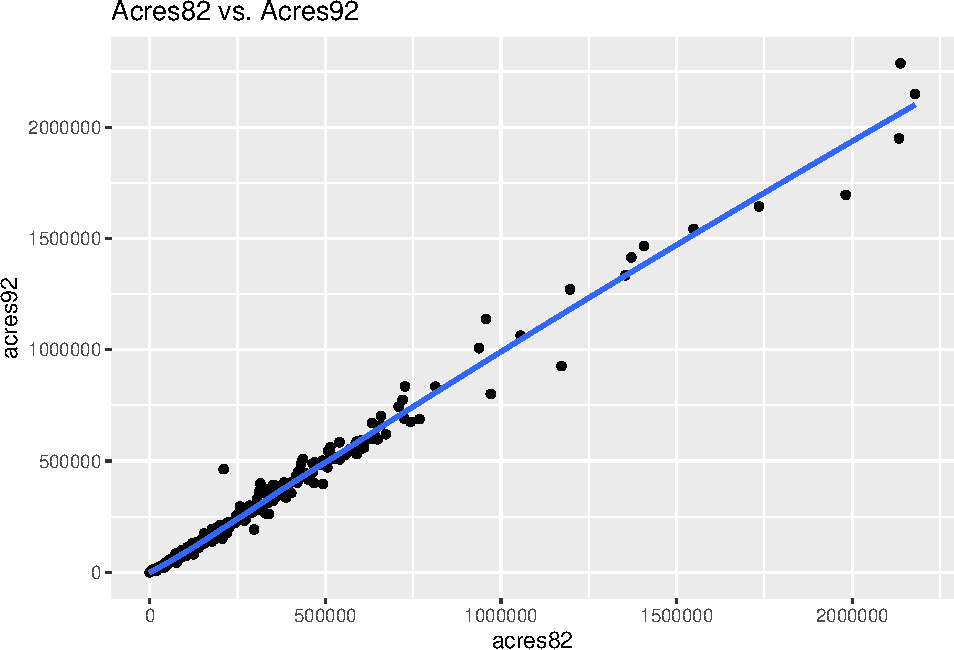
\includegraphics{homework7_files/figure-latex/unnamed-chunk-5-1.pdf}
\[logit = -1.20031411 - 0.03464716(Dose)\]
\[logit(dose = 0) = -1.20031411 - 0.03464716(0) = -1.20031411\]
\[logit(dose = 0.25) = -1.20031411 - 0.03464716(0.25) = -1.208976\]
\[logit(dose = 1) = -1.20031411 - 0.03464716(1) = -1.234961\]
\[logit(dose = 2) = -1.20031411 - 0.03464716(2) = -1.269608\]

\begin{enumerate}
\def\labelenumi{\alph{enumi}.}
\setcounter{enumi}{1}
\item
  \newline
\end{enumerate}

\begin{center}\rule{0.5\linewidth}{0.5pt}\end{center}

\hypertarget{problem-4-death-penalty-and-race-ch.-21-exercise-10-a-e}{%
\subsection{Problem 4: Death Penalty and Race: ch.~21 exercise 10
(a-e)}\label{problem-4-death-penalty-and-race-ch.-21-exercise-10-a-e}}

This data set is \texttt{case1902}.

\begin{Shaded}
\begin{Highlighting}[]
\NormalTok{case1902 }\OtherTok{\textless{}{-}}\NormalTok{ case1902}
\NormalTok{case1902\_glm }\OtherTok{\textless{}{-}} \FunctionTok{glm}\NormalTok{(Death}\SpecialCharTok{/}\NormalTok{(Death}\SpecialCharTok{+}\NormalTok{NoDeath) }\SpecialCharTok{\textasciitilde{}}\NormalTok{ Aggravation, }\AttributeTok{family =}\NormalTok{ binomial, }\AttributeTok{weights =}\NormalTok{ NoDeath }\SpecialCharTok{+}\NormalTok{ Death, }\AttributeTok{data =}\NormalTok{ case1902)}
\end{Highlighting}
\end{Shaded}

\begin{center}\rule{0.5\linewidth}{0.5pt}\end{center}

\hypertarget{problem-5-space-shuttle-challenger-article-assigned-reading}{%
\subsection{Problem 5: Space Shuttle Challenger (article assigned
reading)}\label{problem-5-space-shuttle-challenger-article-assigned-reading}}

The data set \texttt{challenger.csv} contains the o-ring data presented
in Table 1 of the Dalal, Fowlkes, and Hoadley paper. The observations
(rows) in this data set are flights taken under various conditions. The
variables are \texttt{temperature} (ambienent temp in Farenheit),
\texttt{pressure} (field leak-check pressure), \texttt{nozzle.pres}
(nozzle leak-check pressure), \texttt{damaged} (number of damaged
o-rings); \texttt{number} (number of o-rings each launch), and
\texttt{incident} (indicates whether at least one o-ring was damaged (1)
or if no o-rings were damaged (0)).

\begin{Shaded}
\begin{Highlighting}[]
\NormalTok{chall }\OtherTok{\textless{}{-}} \FunctionTok{read.csv}\NormalTok{(}\StringTok{"http://people.carleton.edu/\textasciitilde{}kstclair/data/challenger.csv"}\NormalTok{)}
\end{Highlighting}
\end{Shaded}

\hypertarget{a-recreate-figure-1b-by-plotting-the-number-of-damaged-o-rings-vs.-temperature.-you-will-need-to-jitter-the-points-since-some-overlap-so-use-geom_jitterheight-.05.-why-does-omitting-the-0-damage-incident-flights-figure-1a-obscure-the-relationship-between-temperature-and-o-ring-performance}{%
\subsubsection{\texorpdfstring{(5a) Recreate Figure 1b by plotting the
number of damaged o-rings vs.~temperature. You will need to jitter the
points since some overlap so use \texttt{geom\_jitter(height\ =\ .05)}.
Why does omitting the 0 damage incident flights (Figure 1a) obscure the
relationship between temperature and o-ring
performance?}{(5a) Recreate Figure 1b by plotting the number of damaged o-rings vs.~temperature. You will need to jitter the points since some overlap so use geom\_jitter(height = .05). Why does omitting the 0 damage incident flights (Figure 1a) obscure the relationship between temperature and o-ring performance?}}\label{a-recreate-figure-1b-by-plotting-the-number-of-damaged-o-rings-vs.-temperature.-you-will-need-to-jitter-the-points-since-some-overlap-so-use-geom_jitterheight-.05.-why-does-omitting-the-0-damage-incident-flights-figure-1a-obscure-the-relationship-between-temperature-and-o-ring-performance}}

\hypertarget{b-the-first-regression-model-considered-in-section-3.1-was-a-regression-for-the-number-of-damaged-o-rings.-given-a-particular-temperature-and-pressure-x-values-we-model-y-the-number-damaged-as-a-binomial-random-variable-with-parameters-m-and-pix.-what-is-m-equal-to-for-this-model-what-is-pix-the-probability-of}{%
\subsubsection{\texorpdfstring{(5b) The first regression model
considered in section 3.1 was a regression for the number of damaged
o-rings. Given a particular temperature and pressure (X-values), we
model \(Y=\) the number damaged as a binomial random variable with
parameters \(m\) and \(\pi(X)\). What is \(m\) equal to for this model?
What is \(\pi(X)\) the probability
of?}{(5b) The first regression model considered in section 3.1 was a regression for the number of damaged o-rings. Given a particular temperature and pressure (X-values), we model Y= the number damaged as a binomial random variable with parameters m and \textbackslash pi(X). What is m equal to for this model? What is \textbackslash pi(X) the probability of?}}\label{b-the-first-regression-model-considered-in-section-3.1-was-a-regression-for-the-number-of-damaged-o-rings.-given-a-particular-temperature-and-pressure-x-values-we-model-y-the-number-damaged-as-a-binomial-random-variable-with-parameters-m-and-pix.-what-is-m-equal-to-for-this-model-what-is-pix-the-probability-of}}

\hypertarget{c-fit-the-logistic-regression-of-damaged-on-temperature-and-pressure.-you-can-verify-that-your-coefficient-estimates-ses-and-residual-deviance-match-the-articles-numbers-pg.-948.-is-temperature-significance-after-accounting-for-pressure-is-pressure-significance-after-accounting-for-temperature}{%
\subsubsection{\texorpdfstring{(5c) Fit the logistic regression of
\texttt{damaged} on \texttt{temperature} and \texttt{pressure}. (You can
verify that your coefficient estimates, SEs, and residual deviance match
the article's numbers (pg. 948).) Is temperature significance after
accounting for pressure? Is pressure significance after accounting for
temperature?}{(5c) Fit the logistic regression of damaged on temperature and pressure. (You can verify that your coefficient estimates, SEs, and residual deviance match the article's numbers (pg. 948).) Is temperature significance after accounting for pressure? Is pressure significance after accounting for temperature?}}\label{c-fit-the-logistic-regression-of-damaged-on-temperature-and-pressure.-you-can-verify-that-your-coefficient-estimates-ses-and-residual-deviance-match-the-articles-numbers-pg.-948.-is-temperature-significance-after-accounting-for-pressure-is-pressure-significance-after-accounting-for-temperature}}

\hypertarget{d-conduct-a-goodness-of-fit-test-for-the-part-c-model.-do-we-have-any-evidence-for-extra-binomial-variation-can-we-trust-this-test-result-e.g.-are-the-assumptions-needed-to-trust-this-test-met}{%
\subsubsection{(5d) Conduct a goodness-of-fit test for the part (c)
model. Do we have any evidence for extra-binomial variation? Can we
trust this test result? (e.g.~are the assumptions needed to trust this
test
met?)}\label{d-conduct-a-goodness-of-fit-test-for-the-part-c-model.-do-we-have-any-evidence-for-extra-binomial-variation-can-we-trust-this-test-result-e.g.-are-the-assumptions-needed-to-trust-this-test-met}}

\hypertarget{e-fit-the-logistic-regression-of-damaged-on-temperature-and-use-this-model-to-plot-the-estimated-probability-of-o-ring-failure-as-a-function-of-temperature-for-temps-ranging-from-30-to-90-degrees.-to-extend-the-geom_smooth-to-these-limits-add-the-layers-xlim30-90-ylim01-before-the-geom_smooth-and-add-the-argument-fullrangetrue-to-geom_smooth.}{%
\subsubsection{\texorpdfstring{(5e) Fit the logistic regression of
\texttt{damaged} on \texttt{temperature} and use this model to plot the
estimated probability of o-ring failure as a function of temperature for
temps ranging from 30 to 90 degrees. To extend the \texttt{geom\_smooth}
to these limits, add the layers \texttt{xlim(30,\ 90)\ +\ ylim(0,1)}
\emph{before} the \texttt{geom\_smooth} and add the argument
\texttt{fullrange=TRUE} to
\texttt{geom\_smooth}.}{(5e) Fit the logistic regression of damaged on temperature and use this model to plot the estimated probability of o-ring failure as a function of temperature for temps ranging from 30 to 90 degrees. To extend the geom\_smooth to these limits, add the layers xlim(30, 90) + ylim(0,1) before the geom\_smooth and add the argument fullrange=TRUE to geom\_smooth.}}\label{e-fit-the-logistic-regression-of-damaged-on-temperature-and-use-this-model-to-plot-the-estimated-probability-of-o-ring-failure-as-a-function-of-temperature-for-temps-ranging-from-30-to-90-degrees.-to-extend-the-geom_smooth-to-these-limits-add-the-layers-xlim30-90-ylim01-before-the-geom_smooth-and-add-the-argument-fullrangetrue-to-geom_smooth.}}

\hypertarget{f-use-your-model-from-part-e-to-predict-the-probability-that-an-o-ring-fails-at-a-temperature-of-31-degrees-the-temp-the-morning-of-the-challenger-launch.-knowing-that-o-ring-failure-can-result-in-catastrophic-damage-would-you-have-advised-nasa-to-launch-the-challenger-that-morning}{%
\subsubsection{(5f) Use your model from part (e) to predict the
probability that an o-ring fails at a temperature of 31 degrees (the
temp the morning of the Challenger launch). Knowing that o-ring failure
can result in catastrophic damage, would you have advised NASA to launch
the Challenger that
morning?}\label{f-use-your-model-from-part-e-to-predict-the-probability-that-an-o-ring-fails-at-a-temperature-of-31-degrees-the-temp-the-morning-of-the-challenger-launch.-knowing-that-o-ring-failure-can-result-in-catastrophic-damage-would-you-have-advised-nasa-to-launch-the-challenger-that-morning}}

\end{document}
